\documentclass{beamer}
\title{Exploration of Protein Phenotypes}
\author{Alvaro Barbeira}
\usepackage[utf8]{inputenc}
\usepackage{default}
\usepackage{graphicx}
\usetheme{Warsaw}

\begin{document}
  %title
  \begin{frame}
    \titlepage
  \end{frame}
  \begin{frame}
    \frametitle{Outline}
    \tableofcontents
  \end{frame}
  %intro
  \section{Problem Introduction}
  \begin{frame}
    \frametitle{Problem:}
    \framesubtitle{Genomics of Proteins}
    \begin{itemize}
      \item
      Heritability of proteins was chosen as study subject because there are not many published results about it.
      \item
      Low data quality and noise was expected.
      \item
      Chosen data sets: hapmap release 23, Protein Data from Ron Hause and Lingfeng Wu.
      \item
      Correlations between Gene expression and Protein were also studied, using PrediXcan data.
    \end{itemize}
  \end{frame}
  
  \section{Heritability}
  
  \begin{frame}
    \frametitle{General Method}
    The basic procedure was:
    \begin{itemize}
      \item
      Selecting individuals that satisfied $MAF >= 0.05$ with plink 1.07
      \item
      Generating Genetic Relationship Matrix with GCTA 1.24.4
      \item
      Using GCTA to figure out Restricted Maximum Likelihood (REML) for each protein
    \end{itemize}
    \vskip15pt
    Results:
    Heritability took values either $0$ or $1$ for most genes, with standard error near $~1$.
  \end{frame}
  
  \begin{frame}
    \frametitle{Data from Hause et al results}
    \begin{center}
      \begin{figure}
      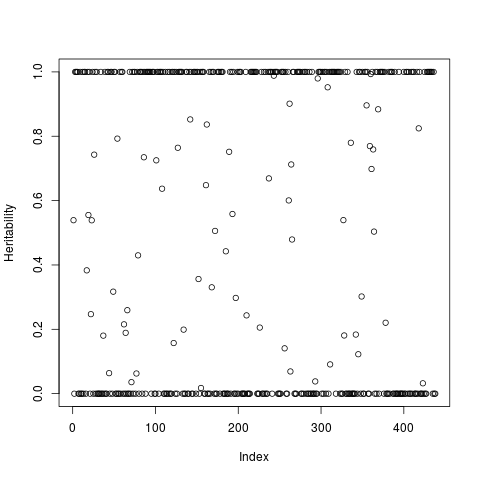
\includegraphics[scale=0.3]{../Out/reml_hause.png}
      \caption{Heritability of Hause Gene Data}
      \end{figure}
    \end{center}
  \end{frame}
  
  \begin{frame}
    \frametitle{Data from Wu et al results}
    \begin{center}
      \begin{figure}
      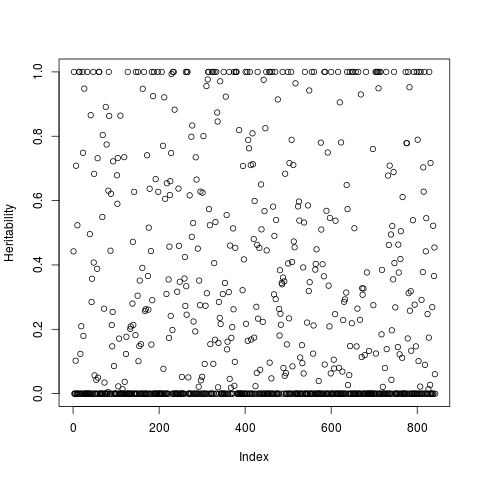
\includegraphics[scale=0.3]{../Out/reml_wu.png}
      \caption{Heritability of Wu Gene Data}
      \end{figure}
    \end{center}
  \end{frame}
  
  \section{mRNA Levels/Gene Expresion vs Protein}
    \begin{frame}
    \frametitle{General Method}
    The procedure consisted in:
    \begin{itemize}
      \item
      Taking protein values for chosen people in the previous experiment.
      \item
      Figuring out correlation to mRNA levels (gene expression) data generated by PrediXcan.
      \item
      Since several proteins might correspond to a single gene, 
      two phenotypes were studied: each protein on its own against its corresponding gene, 
      and average of all proteins for a single gene.
    \end{itemize}
    \vskip15pt
    Results:
    $R^2$ taken as correlation indicator was not great, but showed that some relationship could be picked up in spite of the noise.
    Values near $1$ are taken by sets where very few individuals' data was available.
  \end{frame}
  
  \begin{frame}
    \frametitle{Data from Hause et al results}
    \begin{center}
      \begin{figure}
      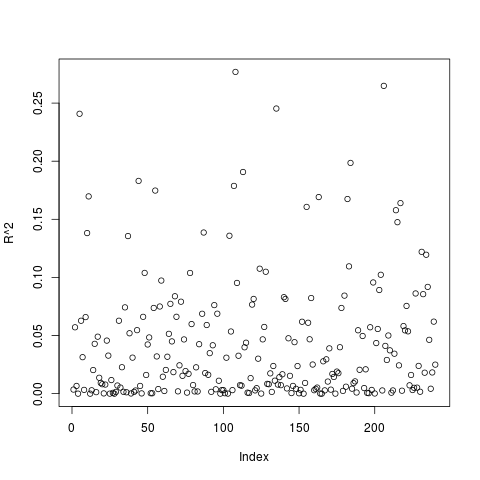
\includegraphics[scale=0.3]{../Out/hause-mrna-protein-r-squared.png}
      \caption{Correlation ($R^2$) for Hause et al. data}
      \end{figure}
    \end{center}
  \end{frame}

  \begin{frame}
    \frametitle{Data from Hause et al results}
    \begin{center}
      \begin{figure}
      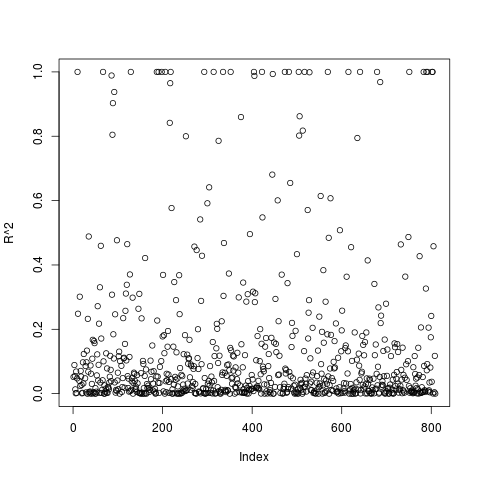
\includegraphics[scale=0.3]{../Out/wu-mrna-protein-r-squared.png}
      \caption{Correlation ($R^2$) for Wu et al. data}
      \end{figure}
    \end{center}
  \end{frame}

  \section{Bonus track: Predixcan vs Affymetrix gene expression}
  \begin{frame}
    \frametitle{PrediXcan vs Affymetrix data}
    As a last check, predixcan data was compared to measured gene expresion from affymetrix.
    \begin{itemize}
      \item
      Affymetrix data had a many-to-many relationship between genes and expression measurement, so a single $(gene,measurement)$ pair was chosen for each set
      \item
      Correlation between predixcan values and affymetrix measurements were figured out
    \end{itemize}
    \vskip15pt
    Results:
    Again, $R^2$ was not great, but showed some relationship
    Values near $1$ are taken by sets with very few individuals' data was available.
  \end{frame}
  
  \section{Possible Next Steps}
  \begin{frame}
    \frametitle{}
    Things to try if suddenly found idle on a sunday afternoon without anything else to do:
    \begin{itemize}
      \item
      Take again on heritability using protein eigenvectors as covariates in gcta
      \item
      Use PrediXcan to predict protein levels and correlate to measured proteins
      \item
      Surrogate Variable Analysis of protein data
      \item
      Figure out PCA analysis of proteins, and study heritability of residuals
    \end{itemize}
  \end{frame}
\end{document}
